\subsection{CMOS 器件模型:等效电路分解+动态参数}\label{subsec:cmos-model}
如前文所述,任何符合假设\ref{assumption:intrinsic-params-dependencies}
的子电路模块,例如 CMOS 管,都可基于 SubModel 机制建模为“等效电路分解+动态参数”,
这一节我们就提供一个基于查找表实现的示例。
需说明的是,更兼容现有技术的做法应该是直接
在 SubModel 中重新实现 BSIM 模型\cite{chauhan2012bsim},这在本文不涉及。
CMOS 模块示例的具体定义可参考附录\hyperref[appendix:mos-subckt]{B},
它在 AC 分析下的等效电路图为图\ref{fig:mos-small-signal-model-2},
其定义的基本要素如下
\begin{figure}[htpb]
  \centering
  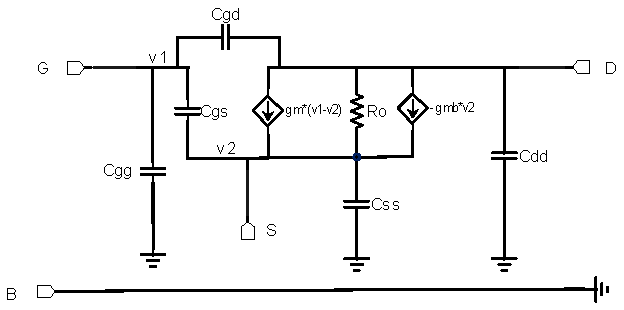
\includegraphics[width=0.7\textwidth]{fig/mos-small-signal-model-2.pdf}
  \caption{CMOS 等效小信号模型,参考\cite[Figure 2.39]{razavi2002design}。
  这里 Ro 是阻值为 $\frac{1}{\text{GDS}}$ 的电阻器。}
  \label{fig:mos-small-signal-model-2}
\end{figure}
\begin{enumerate}[partopsep=0pt,topsep=0pt,itemsep=0pt,parsep=0pt]
  \item 内外节点是 \textbf{nodes}=[gate,source,drain,bulk]。
  \item 输入变量即该器件尺寸 \textbf{ip}=[MosL,MosW]。
  \item SubModel 输出的内部变量
    \textbf{intrp}=[ID,GDS,CDD,CSS,CGG,CGS,CGD,GM,GMB]
    值由 \textbf{nodes} 四端偏置电压及器件尺寸\textbf{ip}决定。
\end{enumerate}
编译器读取该模块定义后,
将加载外部库并生成一个 “lut.MosLookup” 类型的函数对象作为 SubModel 注册到
子电路规则(表\ref{tab:BasicCompositeSubCktRule})中。
内部变量 ID 表示 DC 分析下 source,drain 之间的直流电流,
GDS,CDD,GM 等则是 AC 分析下的等效小信号参数,其中
\begin{enumerate}[partopsep=0pt,topsep=0pt,itemsep=0pt,parsep=0pt]
  \item 内置基本器件 ICS,ACVCCS (附录\hyperref[appendix:mos-subckt]{B})
    的作用是使得 ID 仅在 DC 分析下起作用,
    而 GDS,GM,GMB 仅在 AC 分析下起作用。
  \item 方程构建器的 DCAC 混合分析或 DC 分析计算图可运行此电路模块,
    但 AC 分析计算图不可单独运行此电路模块:
    要建立 AC 分析方程需先计算由 DC 偏置电压决定的 [GDS,GM] 等,
    这与直接通过 TRAN 分析方程诱导出小信号线性方程不同
    (附录\hyperref[appendix:TRAN-to-AC-equation]{A})。
    事实上,假设\ref{assumption:intrinsic-params-dependencies} 中也规定,
    内部变量可依赖于偏置电压信号,而不可依赖于线性分析中的小信号。
  \item SubModel 可在确保遵循相应自动微分系统的接口要求的前提下,
    自由调用外部程序,例如使用三维样条插值。
\end{enumerate}
从示例说明中可以看出,基于 SubModel 机制的 “等效电路分解+动态参数”
器件模型表示法具有如下优势
\begin{enumerate}[partopsep=0pt,topsep=0pt,itemsep=0pt,parsep=0pt]
  \item SubModel 与电路的网络分析、仿真是相互解耦的,它只负责
    内部变量及 Jacobian 矩阵的计算(Sec \ref{subsec:subckt-instance-data-structure}),
    无需关心电路连接关系。
  \item SubModel 计算内部变量的语法及能力边界取决于编译器对网表中
    “SubModel”字段的处理,实现上可考虑借助各类外部程序及自动微分工具。
\end{enumerate}
\subsection{运算放大器尺寸寻优:多 PVT 下器件DC工作状态优化}
模拟电路设计的尺寸寻优流程如图\ref{fig:manually-design},
设计师将目标工艺提供的可用器件连接成各类电路,
并基于一定的方法论和经验调节器件如 CMOS 管的尺寸(即Device Sizing)
使得电路可在给定面积、功耗约束下达成各类指标,
这期间需反复使用电路仿真来定量了解电路行为及性能,而无需实际制造。
\begin{figure}[htpb]
  \centering
  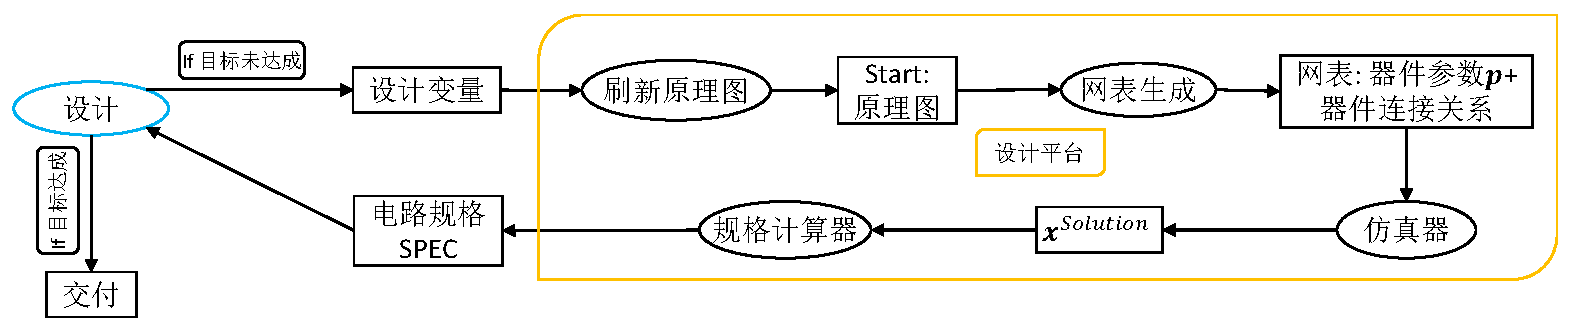
\includegraphics[width=\textwidth]{fig/manually-design.pdf}
  \caption{尺寸寻优:人工迭代流程}
  \label{fig:manually-design}
\end{figure}

这个流程可自然的转换成优化问题来求解,
根据梯度是否可获取,可采取不同的优化策略
\cite{zhan2004optimization,agrawal2006circuit,huang2013efficient,
nieuwoudt2005multi,peng2016efficient,girardi2011analog,lyu2018batch,
wang2014enabling,lyu2017efficient,tang2018parametric}。
为了获取梯度,以 DC 仿真为例:直流稳态方程组
$\bm{F}(\bm{x},\bm{p})=\bm{0}$ 自然地给出了参数 $\bm{p}$
到方程组的解 $\bm{x}^{solution}$ 的隐式映射,该映射的 Jacobian 矩阵为
$\nabla_{\bm{p}}\bm{x}^{solution}=-\nabla_{\bm{x}}\bm{F}\backslash\nabla_{\bm{p}}\bm{F}$,
而 $\nabla_{\bm{x}}\bm{F},\nabla_{\bm{p}}\bm{F}$ 可由 Sec \ref{sec:Joanna}
介绍的方程组构建方法(计算图\ref{fig:computational-graph}) 直接给出。
借助这些信息,我们可以使用梯度优化方法(图\ref{fig:solve-then-optimize})。
注意,实际优化过程中,无需完整求解 $\nabla_{\bm{x}}\bm{F}$ 的逆,
只需要对给定的损失函数或约束函数 $l$,在每次迭代的梯度反传时求解线性方程组即可:
$\nabla_{\bm{p}}l(\bm{x}^{solution})=(\nabla_{\bm{p}}\bm{x})^T\cdot\nabla_{\bm{x}}l
=-(\nabla_{\bm{p}}\bm{F})^T\cdot\big(\nabla_{\bm{x}}\bm{F}^T\backslash\nabla_{\bm{x}}l\big)$
\begin{figure}[htpb]
  \centering
    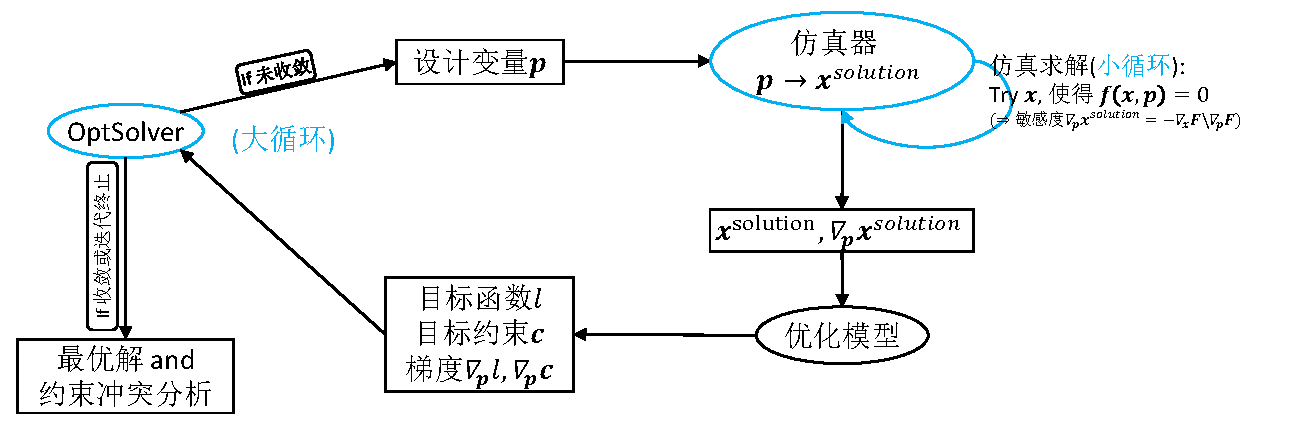
\includegraphics[width = 0.7\textwidth]{fig/solve-then-optimize.pdf}
  \caption{尺寸自动寻优}
  \label{fig:solve-then-optimize}
\end{figure}

\begin{figure}[htbp]
  \centering
  \begin{subfigure}{0.3\textwidth}
    \includegraphics[width=\textwidth]{fig/amplifier-diagram.png}
    \caption{运算放大器示意图\cite{OpAmpPNG}}
    \label{subfig:amplifier-diagram}
  \end{subfigure}
  \begin{subfigure}{0.65\textwidth}
    \includegraphics[width=\textwidth]{fig/amplifier-transfer-function.png}
    \caption{尺寸优化后,运放的输入输出频响曲线}
    \label{subfig:amplifier-transfer-function}
  \end{subfigure}
  \caption{\textbf{左(a)}:运算放大器示意图,内部包含偏置电路及主电路
  共17个n-MOSFET和17个p-MOSFET。
  在 DC 工作点下,可以在 $V_+,V_-$ 输入角频率 $\omega$ 的扰动小信号,
  从$V_{out}$处可以检测到输出信号。 \textbf{右(b)}:尺寸优化后,
  运放在 $Corner=tt,Temperature=27$
  工作条件下的频响曲线。 其中 va4,va5 是电路中的两个内部节点。}
\end{figure}
以一个运算放大器(图\ref{subfig:amplifier-diagram})为例,我们把该电路中各设计变量
即所有 MOS 管的沟道长和宽作为待优化变量。
给定外部电流电压源 Ibias0,Ibias1 及 $V_{dd},V_+,V_-$,以及负载电阻电容
$R_L=200\Omega,C_L=10^{-10}\text{F}$,这里我们设置的指标如下,
\begin{enumerate}[partopsep=0pt,topsep=0pt,itemsep=0pt,parsep=0pt]
  \item 在 $Corner\in[tt,ff,ss],Temperature\in[27,-40,125]$ 共 9 种工作条件下,
    要求所有 MOS 管的 DC 工作状态均为饱和,以 NMOS 管为例,其 DC 偏置电压应满足
    \vspace{-1em}
    \[
      \min(V_{gs},V_{ds},V_{sb},V_{gs}-V_{th})\geq0.
      \vspace{-1em}
    \]
    其中 $V_{th}$ 依赖于 MosL,$V_{gs},V_{ds}$。
    对不同工作条件 SubModel 需加载不同的数据库,最终得到的仿真解也各有区别。
  \item 在典型工作条件 $Corner=tt,Temperature=27$ 下,允许 $V_+,V_-$
    电压源有上下浮动,但需满足关系 $V_++V_-=5v$,
    此时,$V_{out}$ 的DC 偏置工作点作为 $V_+,V_-$ 的函数,
    要求其最大值大于 4.35v,最小值小于 0.3v,
    这一要求类似于电路的输出摆幅指标。
  \item 在典型工作条件 $Corner=tt,Temperature=27$ 下,对电路进行 AC 分析,
    在 $V_+,V_-$ 处输入 $v_{in+},v_{in-}=\pm0.5$ 的信号,
    要求 $V_{out}$ 的直流增益 $gain=20\cdot\log_{10}(|v_{out}|)$ 达到100。
  \item 各器件设计变量满足事先规定的对称性约束,例如输入对管
    $M_{n0\_in},M_{n0\_ip}$ 的尺寸 MosL,MosW 应完全相等,电流境
    $M_{p30\_mirr},M_{p20\_mirr},M_{p10\_mirr},M_{p50\_mirr},M_{p60\_mirr}$
    的沟道长 MosL 应相等,等等。
\end{enumerate}
\begin{equation}\label{eq:optimization}
  \begin{split}
    \min_{\bm{p}} l &= \max(5-\log_{10}(|\bm{v}[out]|),0)^2 \\
    \st \ \ \ \ \ \ 
    & \forall c\in[tt,ff,ss],t\in[27,-40,125], \\
    & \ \ \ \ \bm{x}_L\preceq\bm{x}^{c,t}\preceq\bm{x}_U;
    Saturation(\bm{x}^{c,t},\bm{p})\succeq\bm{0}; \\
    & \bm{x}^{down}[out]\leq0.3;\bm{x}^{up}[out]\geq4.35; \\
    & \bm{v}=\bm{A}^{tt,27}\backslash\bm{b}^{tt,27}; \ C\cdot\bm{p}=\bm{0}.
  \end{split}
\end{equation}
我们将上述设计任务表述为约束优化问题 Prob.\eqref{eq:optimization}。
其中 $\bm{p}\to\{\bm{x}^{c,t}\},\bm{x}^{down},\bm{x}^{up}$
通过求解对应工作条件及输入偏置 $V_+,V_-$ 下的 DC 方程组得到;
$\bm{v}=\bm{A}^{tt,27}\backslash\bm{b}^{tt,27}$ 是求解
$Corner=tt,temperature=27$ 时 AC 分析线性方程组,
其中的系数实际上就是依赖于 $\bm{x}^{tt,27},\bm{p}$ 的各器件的
GM,GDS 等等。
我们可借助 DCAC 混合分析的计算图来计算
$\bm{A},\bm{b},\nabla_{\bm{x}}\bm{A},\nabla_{\bm{x}}\bm{b}$
\footnote{$A=i\omega\cdot\nabla_{\bm{x}}\bm{Q}+\nabla_{\bm{x}}\bm{F}$,
但这里使用 DCAC 计算图而非 $\nabla\bm{Q},\nabla\bm{F}$ 来计算 $\nabla A$,
否则需计算和反传 $\bm{Q},\bm{F}$ 关于 $\bm{x}$ 的二阶导,
这将大大增加计算图实现难度},
进一步可获得 $\nabla_{\bm{x}}l,\nabla_{\bm{p}}l$
(参考附录\hyperref[appendix:inv-linear-equation-grad]{C});
$C\cdot\bm{p}=\bm{0}$ 表示对设计变量的直接约束,例如对称性约束。

优化算法调用开源软件 Ipopt\cite{wachter2006implementation} 实现,
一共包括 72 个待求解变量,27 个等式约束,308 个不等式约束。
整个过程(含 Julia 代码编译加载,网表解析等)在
Intel(R) Core(TM) i7-8700 CPU @ 3.20GHz 使用 6 线程耗时 356 秒,
图\ref{subfig:amplifier-transfer-function} 给出了优化后的电路频响曲线。
从实验结果可以看到,
\begin{enumerate}[partopsep=0pt,topsep=0pt,itemsep=0pt,parsep=0pt]
  \item 基于计算图的层次电路仿真或尺寸寻优,可使得器件模型、求解算法之间
    相互解耦且可灵活的通信。
  \item 计算图中将参数变量化处理,使得许多指标的梯度优化更为简单自然。
\end{enumerate}
最后需要说明的是,上述实验仅考虑了各器件的工作状态、电路在典型工作条件下的 DC 增益,
若需进行完整的设计,需在优化问题中引入更多的指标,甚至可能包含离散值指标,
各类指标整合到优化的框架中也并非一蹴而就,这些问题在这里不再详细讨论。
